% #############################################################################
% This is Chapter 4
% !TEX root = ../main.tex
% #############################################################################
% Change the Name of the Chapter i the following line
\fancychapter{Aerial-D Dataset Construction}
\cleardoublepage
% The following line allows to ref this chapter
\label{chap:implement}

This section details our comprehensive approach to constructing Aerial-D, a large-scale referring expression segmentation dataset for aerial imagery. Our methodology combines automated rule-based expression generation with a multimodal LLM expression component that is preceded by a cost-efficient distillation step, enabling both scale and linguistic diversity. We begin by establishing our source datasets, then describe our rule-based pipeline for generating referring expressions from existing annotations, followed by our distilled large language model enhancement procedure, and conclude with comprehensive dataset statistics demonstrating the scope and characteristics of the final resource.

% #############################################################################
\section{Source Datasets}

The Aerial-D dataset is constructed from two complementary aerial datasets with different annotation styles: iSAID (instance segmentation) and LoveDA (semantic segmentation), as illustrated in Table~\ref{tab:dataset_sources}.


% Dataset sources table with images
\begin{table}[H]
\centering
\caption{Source Dataset Characteristics}
\label{tab:dataset_sources}
\begin{tabular}{@{}p{4cm}p{8cm}@{}}
\toprule
\multicolumn{2}{c}{\textbf{iSAID Dataset}} \\
\midrule
\raisebox{-0.5\height}{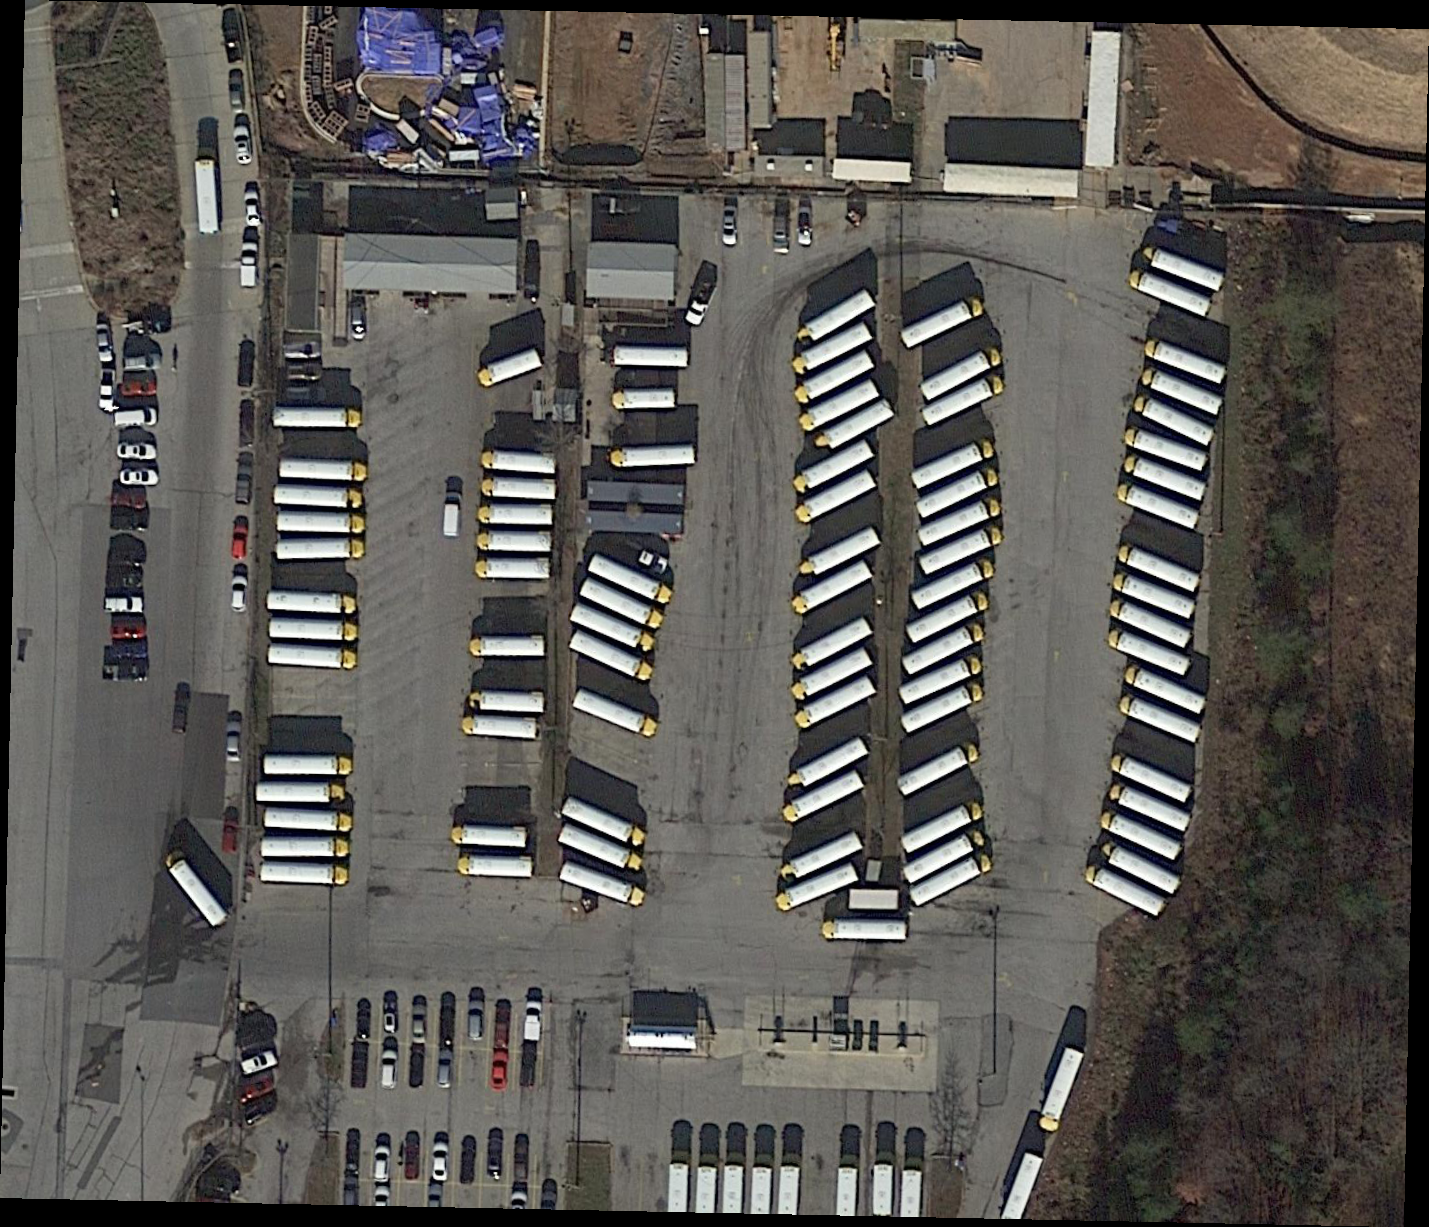
\includegraphics[width=3.5cm, height=3.5cm]{Images/isaid.png}} & 
\hspace{-0.5cm}\parbox[c]{8cm}{\fontsize{10pt}{12pt}\selectfont Contains \textbf{2,806} high resolution images at varying widths of 800 to 13,000 pixels, spatial resolution of \textbf{0.1m to 4.5m}, with \textbf{655,451} instances across \textbf{15} object classes: \textbf{ships}, \textbf{large vehicles}, \textbf{small vehicles}, \textbf{storage tanks}, \textbf{harbors}, \textbf{swimming pools}, \textbf{tennis courts}, \textbf{soccer ball fields}, \textbf{roundabouts}, \textbf{basketball courts}, \textbf{bridges}, \textbf{ground track fields}, \textbf{planes}, \textbf{helicopters}, and \textbf{baseball diamonds}.} \\[0.5cm]
\midrule
\multicolumn{2}{c}{\textbf{LoveDA Dataset}} \\
\midrule
\raisebox{-0.5\height}{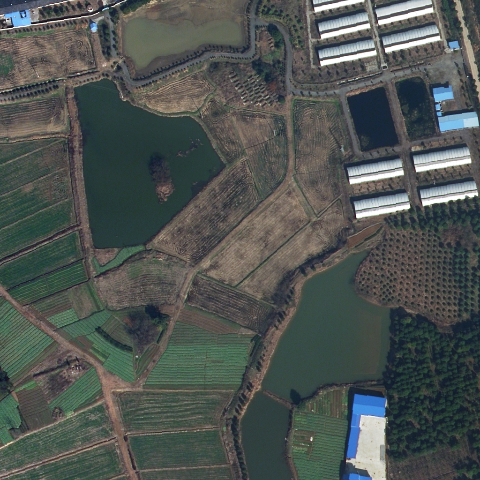
\includegraphics[width=3.5cm, height=3.5cm]{Images/loveda_dataset.png}} & 
\hspace{-0.5cm}\parbox[c]{8cm}{\fontsize{10pt}{12pt}\selectfont Contains \textbf{5,987} images at 1024 pixel width, spatial resolution of \textbf{0.3m}, across \textbf{6} land cover classes: \textbf{building}, \textbf{road}, \textbf{water}, \textbf{barren}, \textbf{forest}, and \textbf{agriculture}.} \\[0.5cm]
\bottomrule
\end{tabular}
\end{table}

We start by putting both sources into the same format so that a single model can learn from them side by side: square patches at 480×480. This size keeps small iSAID objects large enough to describe and segment, while fitting the input expectations of common vision encoders used in our model (e.g., CLIP/SigLIP image towers and SAM backbones\cite{clip,siglip,sam}).

We first resize the 1024×1024 LoveDA tiles directly to 480×480 while preserving their semantic masks. iSAID has uniquely high-resolution imagery with varying aspect ratios, so we instead slide a 480×480 window with overlap across each source image and keep the patches that contain valid instances. After these resizing steps, we run connected-component analysis on LoveDA to turn buildings and water into pseudo-instance targets—these categories tend to appear as isolated structures or bounded water bodies, making them natural candidates for instance-level descriptions. The remaining land-cover classes (e.g., farmland or forest) behave as contiguous surfaces, so we keep them as semantic regions and describe them holistically ("all agricultural land in the image"). The resulting per-patch representation retains instance targets, grouped semantic regions, and the original semantic labels that feed into the subsequent rule-guided expression generation.

% #############################################################################
% #############################################################################
\section{Rule-Based Expression Generation}

The rule-based expression generation pipeline systematically transforms the extracted patches into referring expression datasets through a sequential multi-step process. The pipeline consists of the following key components:

\begin{enumerate}
\item \textbf{Spatial Grid Positioning}: Each 480×480 patch is divided into a three-by-three grid to assign positional attributes such as "in the top right" or "in the center".
\item \textbf{Color Classification}: HSV (Hue-Saturation-Value) color space analysis extracts chromatic and achromatic color descriptors for each object mask, applying confidence thresholds to ensure reliable classification.
\item \textbf{Spatial Relationship Calculation}: An angle-based directional system computes relationships between nearby objects, enabling expressions like "to the left of" or "above".
\item \textbf{Extreme Position Detection}: Identifies instances that occupy boundary locations within their category, such as "the topmost ship" or "the leftmost building".
\item \textbf{Group Formation}: DBSCAN clustering groups nearby instances of the same category to enable collective references such as "the group of 3 ships".
\item \textbf{Expression Synthesis}: Combines all extracted attributes through seventeen distinct expression templates to generate comprehensive referring expressions for each target.
\item \textbf{Uniqueness Filtering}: Identifies and removes duplicate expressions across the dataset, ensuring that each remaining expression uniquely identifies a single object or group and eliminating ambiguous references.
\end{enumerate}

The core challenge is figuring out how to describe these target objects using only what we know from their bounding boxes, masks, and categories. We utilize the bounding box coordinates to understand where each object sits within the image patch. As shown in Figure \ref{fig:rule_example}, we divide each patch into a three-by-three grid marked with dotted lines, so we can say an object is "in the top right" or "in the center". When we have multiple objects of the same type, we also check if any are in extreme positions like the topmost or leftmost instance of that category.

\begin{figure}[t]
\centering
\begin{minipage}{0.5\textwidth}
\centering
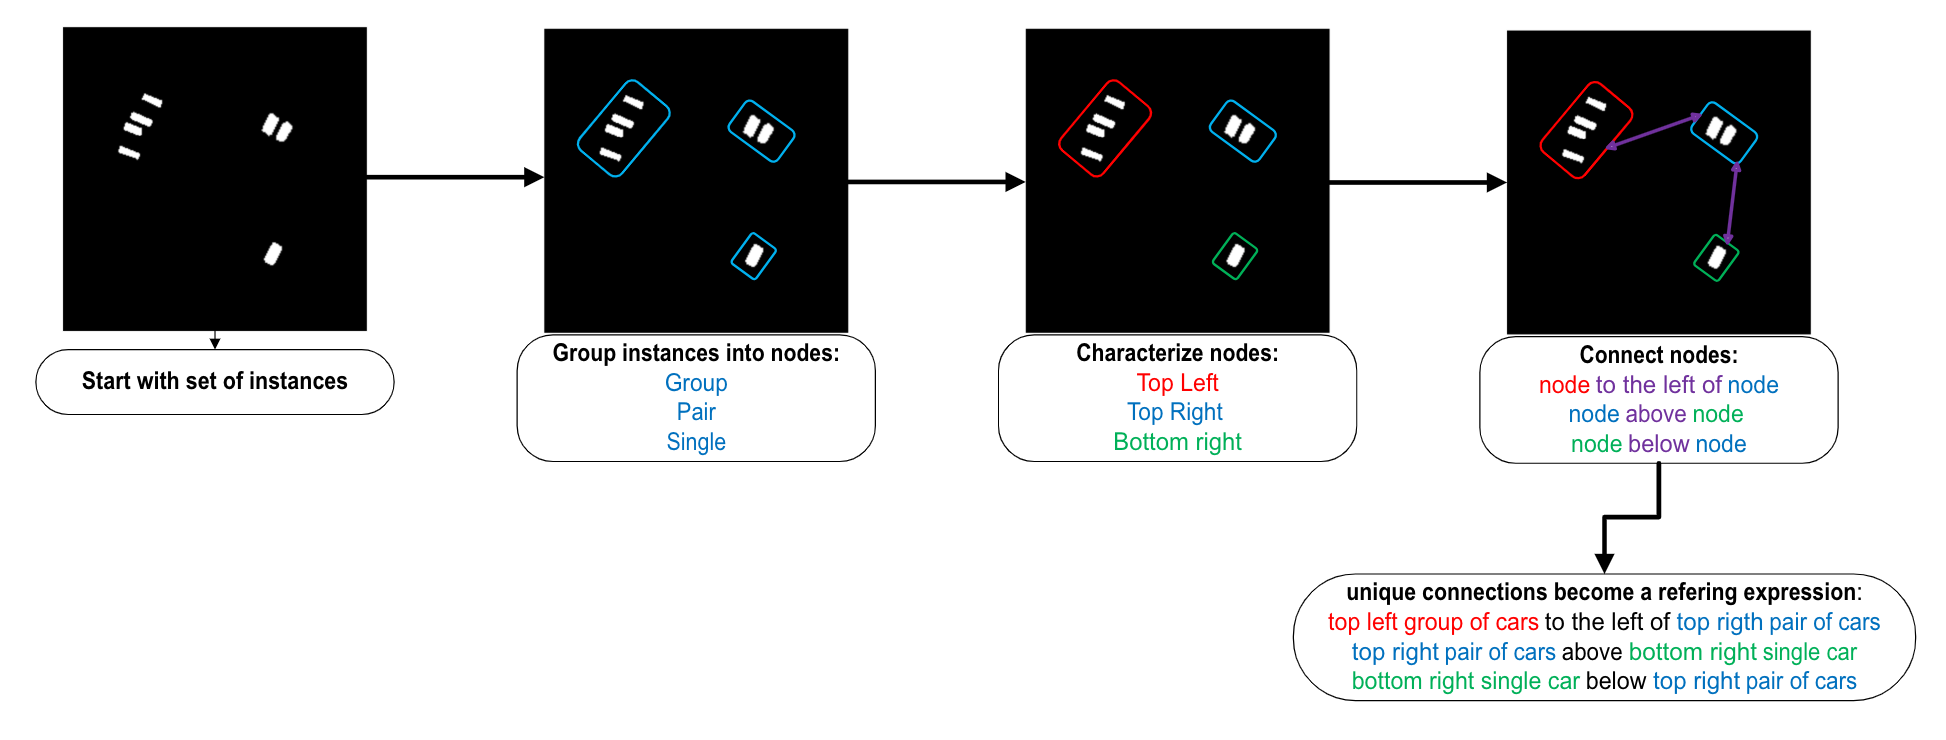
\includegraphics[width=0.7\textwidth]{Images/rule_based_generation.png}
\end{minipage}%
\begin{minipage}{0.5\textwidth}
\centering
\hspace{-1cm}
\raisebox{-0.3\height}{%
\resizebox{\textwidth}{!}{%
\footnotesize
\begin{tabular}{@{}ll@{}}
\toprule
\textbf{Rule Type} & \textbf{Example Instance} \\
\midrule
Category & "plane" \\
Grid Position & "in the top right" \\
Extreme Position & None \\
Color Classification & "light" \\
Directional Relations & "to the bottom right of a plane" \\
& "to the top right of a plane" \\
\midrule
\multicolumn{2}{l}{\textbf{Final Expressions}} \\
\multicolumn{2}{l}{"the plane in the top right"} \\
\multicolumn{2}{l}{"the light plane in the top right"} \\
\multicolumn{2}{l}{"the plane in the top right to the bottom right of a plane"} \\
\multicolumn{2}{l}{"the light plane in the top right to the bottom right of a plane"} \\
\multicolumn{2}{l}{"the plane in the top right to the top right of a plane"} \\
\multicolumn{2}{l}{"the light plane in the top right to the top right of a plane"} \\
\bottomrule
\end{tabular}%
}%
}
\end{minipage}
\caption{Example of rule generation for a single instance. The highlighted plane in the top right section demonstrates how the system assigns spatial, visual, and relational rules that will later be combined into referring expressions.}
\label{fig:rule_example}
\end{figure}

Since we also have the pixel masks for each object, we can analyze their colors by looking at hue–saturation–value (HSV) distributions to distinguish between light and dark objects and a controlled palette of chromatic colors. We require at least 70\% dominance for achromatic labels ("light" or "dark") and a single hue to occupy at least 60\% of the chromatic pixels before we commit to a specific color; otherwise the instance is marked as ambiguous and the colour cue is discarded. This thresholds ambiguous multi-hue regions and helps us ignore noisy signals that would otherwise mislead the language generation. We also avoid using color descriptors for buildings and water since these typically show mixed colors that aren't useful for identification.

We also create relationships between nearby objects by calculating angles between their positions, allowing us to generate expressions like "the ship to the left of the harbor" or "the vehicle above the building". The system uses eight directional relationships: above, below, to the left of, to the right of, and the four diagonal directions.

All these rules combine to generate various referring expressions for each object, as demonstrated in Figure \ref{fig:rule_example} where a single plane generates multiple possible descriptions including "the plane in the top right", "the light plane in the top right", and versions with relational descriptions. However, a significant challenge emerges when multiple objects end up with identical characteristics and generate the exact same expressions, creating ambiguous references where one phrase could describe multiple different objects. We solve this fundamental problem by taking the set of all expressions for all objects and targets in each image, matching them against each other to find duplicates, and when we find expressions that are identical, we cancel both expressions out and discard them as ambiguous. This filtering stage is crucial: it removes targets that cannot be uniquely verbalised using the rules alone, ensures the rule-based component only passes forward unambiguous instances, and guarantees that the downstream dataset never asks models to resolve intentionally ambiguous descriptions.

% Expression uniqueness filter example
\begin{figure}[t]
\centering
\begin{minipage}{0.5\textwidth}
\centering
\includegraphics[width=0.7\textwidth]{Images/filter_unique.png}
\end{minipage}%
\begin{minipage}{0.5\textwidth}
\centering
\hspace{-1cm}
\raisebox{-0.3\height}{%
\resizebox{\textwidth}{!}{%
\footnotesize
\begin{tabular}{@{}ll@{}}
\toprule
\textbf{Expression} & \textbf{Status} \\
\midrule
\multicolumn{2}{l}{\textbf{Object 1 (Light Vehicle)}} \\
\midrule
"the small vehicle in the top right" & \textcolor{red}{Filtered} \\
"the topmost small vehicle" & \textcolor{green!70!black}{Kept} \\
"the light small vehicle in the top right" & \textcolor{green!70!black}{Kept} \\
"the light topmost small vehicle" & \textcolor{green!70!black}{Kept} \\
"the small vehicle in the top right above a small vehicle" & \textcolor{green!70!black}{Kept} \\
\midrule
\multicolumn{2}{l}{\textbf{Object 2 (Dark Vehicle)}} \\
\midrule
"the small vehicle in the top right" & \textcolor{red}{Filtered} \\
"the dark small vehicle in the top right" & \textcolor{green!70!black}{Kept} \\
"the small vehicle in the top right below a small vehicle" & \textcolor{green!70!black}{Kept} \\
\bottomrule
\end{tabular}%
}%
}
\end{minipage}
\caption{Example of expression uniqueness filtering. When two objects share similar attributes, conflicting expressions like "the small vehicle in the top right" are filtered out, while unique expressions that distinguish between objects are retained.}
\label{fig:filter_unique_example}
\end{figure}


% #############################################################################
\section{LLM Expression Generation}
\label{subsec:llm_expression_generation}

While rule-based expression generation provides a solid foundation for referring expression data, these expressions suffer from significant limitations in language variation and visual detail coverage. The rule-based approach produces linguistically constrained expressions with limited wording variations and lacks the ability to reference contextual elements beyond predefined source dataset categories.

To address these limitations, we employ a multimodal Large Language Model (LLM) to enhance our dataset by providing both images and expressions as input, enabling the model to rewrite and improve the original referring expressions. We prompt the LLM with two complementary tasks, as shown in Figure \ref{fig:llm_enhancement_example} and detailed in Appendix~A. The first task focuses on linguistic variation, creating natural language alternatives for each rule-based expression without heavy reliance on visual cues. The second task uses visual information, where the model examines surrounding features in the image around the target object.

To ensure the LLM accurately identifies and describes the target region, we employ a sophisticated visual prompting strategy that adapts to different target types. For discrete objects and groups, we overlay the target region with red bounding boxes that visually highlight the area of interest, guiding the model's attention during generation. Each prompt includes both the full 480×480 image patch and a focused close-up crop centered on the target, which proves essential for small or densely packed objects that might occupy only a few pixels in the original view. For land-cover categories such as vegetation, agriculture, or water that extend across irregular regions without clear bounding boxes, we employ a dual-image prompting technique: the first image shows the original scene with a semi-transparent color overlay masking the target region, while the second image presents the clean unmasked view. This paired presentation helps the LLM anchor its understanding to the relevant semantic region while maintaining awareness of the surrounding context. The combination of bounding box overlays for instance targets, close-up crops for fine details, and dual-image mask prompts for semantic regions ensures the enhancement remains spatially grounded and accurate across all target types in the dataset.

This dual-task prompting transforms basic expressions like "the group of 4 large vehicles in the top center" into linguistically diverse alternatives such as "the cluster of four big vehicles near the upper middle" and visually detailed descriptions like "the four large vehicles lined up side by side just below the pale paved strip at the very top middle", as shown in Figure~\ref{fig:llm_enhancement_example}. The model identifies and references contextual elements not captured in the original datasets, such as the "pale paved strip" and the "grassy area".

% LLM enhancement example figure
\begin{figure}[t]
\centering
\begin{minipage}{0.5\textwidth}
\centering
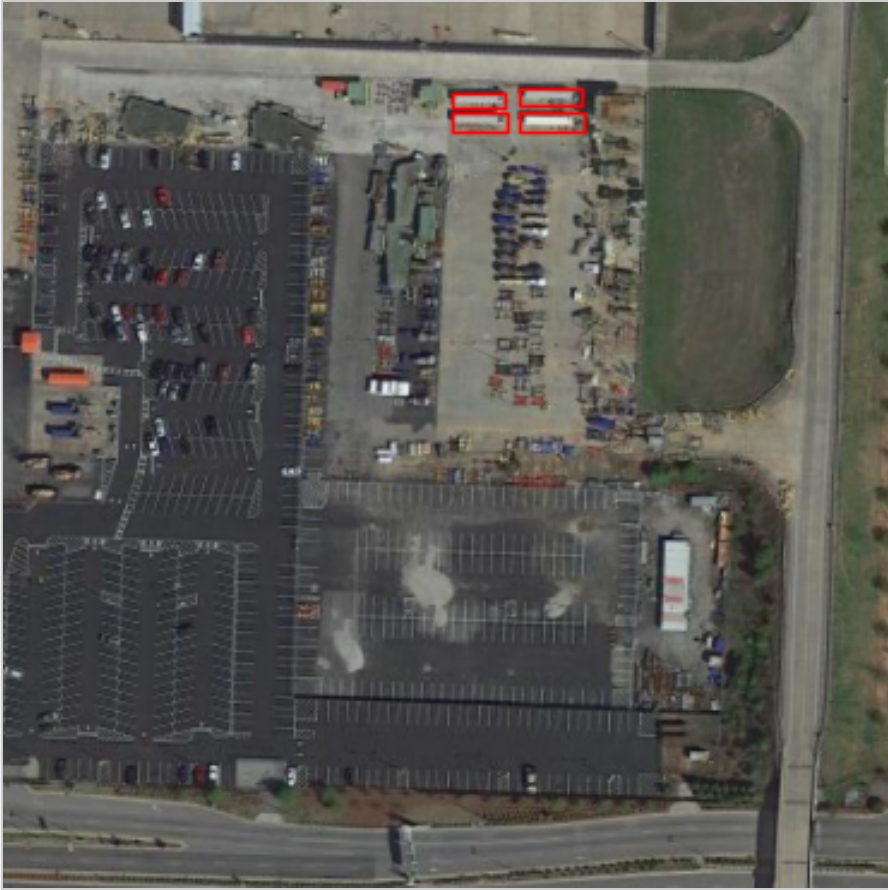
\includegraphics[width=0.7\textwidth]{Images/example_group.png}
\end{minipage}%
\begin{minipage}{0.5\textwidth}
\centering
\hspace{-1cm}
\raisebox{-0.3\height}{%
\footnotesize
\begin{tabular}{@{}p{2cm}p{5cm}@{}}
\toprule
\textbf{Expression Type} & \textbf{Example} \\
\midrule
Original & the group of 4 large vehicles in the top center \\
\midrule
Enhanced & the cluster of four big vehicles near the upper middle \\
\midrule
Unique & the four large vehicles lined up side by side just below the pale paved strip at the very top middle \\
\midrule
Unique & the set of four big vehicles parked in a single row in the upper center beside the grassy area to the right \\
\bottomrule
\end{tabular}%
}
\end{minipage}
\caption{Example of LLM enhancement process showing original aerial image with group of four large vehicles (left) and corresponding expression enhancements (right).}
\label{fig:llm_enhancement_example}
\end{figure}

However, the full dataset contains approximately 300,000 captured targets including both objects and groups. To generate expressions, we process each target individually, meaning we would need 300,000 separate LLM requests. Using production-grade LLMs at this scale—for example, OpenAI's o3 model\cite{o3} with strong visual capabilities—would cost thousands of dollars; Table \ref{tab:cost_comparison} reports the exact breakdown, making direct application prohibitively expensive for research-scale dataset construction.

To address this scalability challenge, we employ a knowledge distillation approach, as illustrated in Figure \ref{fig:llm_distillation}. We utilize OpenAI's o3 model\cite{o3} and compare it against a much more lightweight open‑weights model, Gemma3\cite{gemma3}. We obtain 500 high‑quality outputs from o3 on a representative random subset of targets from the initial dataset. These outputs serve as training data for supervised fine‑tuning using the parameter‑efficient QLoRA method\cite{qlora} on Gemma3‑12B.

During fine-tuning we apply LoRA adapters across both the text decoder and the SigLIP-derived vision stack embedded in Gemma3, which improves instruction adherence, suppresses hallucinations, and stabilises the two-task output schema. The custom-tailored Gemma3 variant can then process all 300,000 targets on a single GPU while honouring the dual-task prompt structure—behaviour the base Gemma3 model fails to follow reliably without distillation. Notably, the distilled model's output quality approaches o3's once fine‑tuned; qualitative comparisons in Figure \ref{fig:distillation_comparison} show closely matched enhancements with markedly reduced hallucinations relative to the base Gemma3 model.

\begin{figure}[t]
\centering
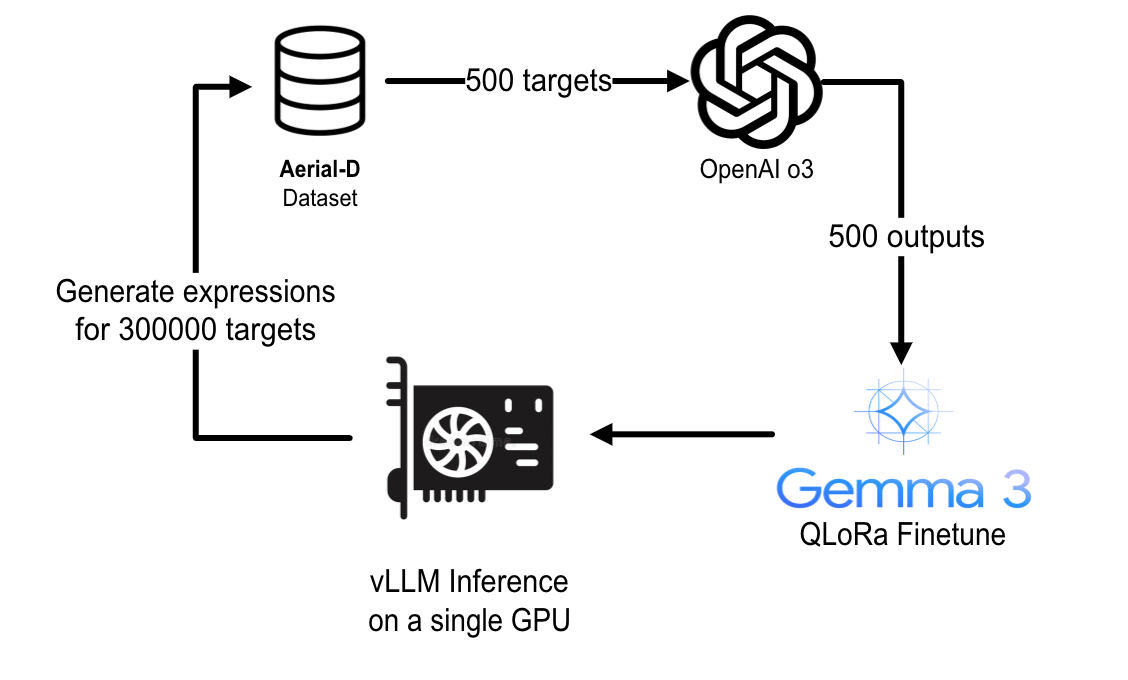
\includegraphics[width=\columnwidth]{Images/distillation.png}
\caption{Knowledge distillation pipeline for scalable LLM enhancement. A small sample of 500 expressions is processed through OpenAI's o3 model\cite{o3} to generate high-quality training targets, which are then used to fine-tune Gemma3‑12B\cite{gemma3} via QLoRA\cite{qlora}. The fine‑tuned model enables cost‑effective local inference to enhance the full dataset using vLLM\cite{vllm} on a single GPU.}
\label{fig:llm_distillation}
\end{figure}

% #############################################################################
\section{Historic Image Filters}
\label{subsec:historic_filters}

In order to keep the dataset useful for models that must operate on archival imagery, we simulate the visual signatures that appear in mid-century aerial collections. Historic film stocks and scanning workflows frequently desaturate colours, compress tonal range, and inject grain, which diminishes the sharp visual cues that modern networks rely upon. To counter this gap between training data and deployment conditions, we apply three parametric transformations that recreate monochrome capture, film fading with grain, and sepia scanning artifacts for every patch.

Let $I_{\text{orig}}(x) \in [0,255]^3$ denote the RGB vector at pixel $x$, and let $\operatorname{clip}(\cdot)$ clamp intensities to the $[0,255]$ range. We first approximate the luminance response of black-and-white film, producing the grayscale target in Equation~\ref{eq:historic_gray}:
\begin{equation}
I_{\text{gray}}(x) = 0.299\,R(x) + 0.587\,G(x) + 0.114\,B(x).
\label{eq:historic_gray}
\end{equation}
Film reproduction is then mimicked by a sequence of tone adjustments. We apply a mild gamma curve in Equation~\ref{eq:historic_gamma}, recenter contrast around the patch mean $\mu$ in Equation~\ref{eq:historic_contrast}, and finally add zero-mean Gaussian noise in Equation~\ref{eq:historic_grain} to replicate silver-halide grain:
\begin{equation}
I_{\gamma}(x) = 255\left( \frac{I_{\text{gray}}(x)}{255} \right)^{\gamma},
\label{eq:historic_gamma}
\end{equation}
\begin{equation}
I_{c}(x) = \big(I_{\gamma}(x) - \mu\big)\,c + \mu,
\label{eq:historic_contrast}
\end{equation}
\begin{equation}
I_{\text{grain}}(x) = \operatorname{clip}\big(I_{c}(x) + \eta(x)\big), \quad \eta(x) \sim \mathcal{N}(0, \sigma^2).
\label{eq:historic_grain}
\end{equation}
The augmentation uses $\gamma = 1.1$, $c = 0.85$, and $\sigma = 0.1\times 255$ so that contrast is gently reduced while a perceptible grain pattern emerges without obscuring object boundaries.

Sepia scanning artifacts are reproduced by applying the linear colour transform in Equation~\ref{eq:historic_sepia}, followed by uniform sensor noise in Equation~\ref{eq:historic_sepia_noise} to emulate digitisation errors:
\begin{equation}
\begin{bmatrix}
S_R(x) \\
S_G(x) \\
S_B(x)
\end{bmatrix}
= \operatorname{clip}\left(
\begin{bmatrix}
0.272 & 0.534 & 0.131 \\
0.349 & 0.686 & 0.168 \\
0.393 & 0.769 & 0.189
\end{bmatrix}
\begin{bmatrix}
R(x) \\
G(x) \\
B(x)
\end{bmatrix}
\right),
\label{eq:historic_sepia}
\end{equation}
where $\mathbf{S}(x) = [S_R(x), S_G(x), S_B(x)]^\top$.
\begin{equation}
I_{\text{sepia}}(x) = \operatorname{clip}\big(\mathbf{S}(x) + \xi(x)\big), \quad \xi(x) \sim \mathcal{U}(0, 50).
\label{eq:historic_sepia_noise}
\end{equation}
Together these transformations compress colour information, soften tonal contrast, and inject characteristic noise while preserving the spatial layout that segmentation relies upon. Figure~\ref{fig:historic_filters} illustrates the qualitative impact on representative patches.

\begin{figure}[H]
\centering
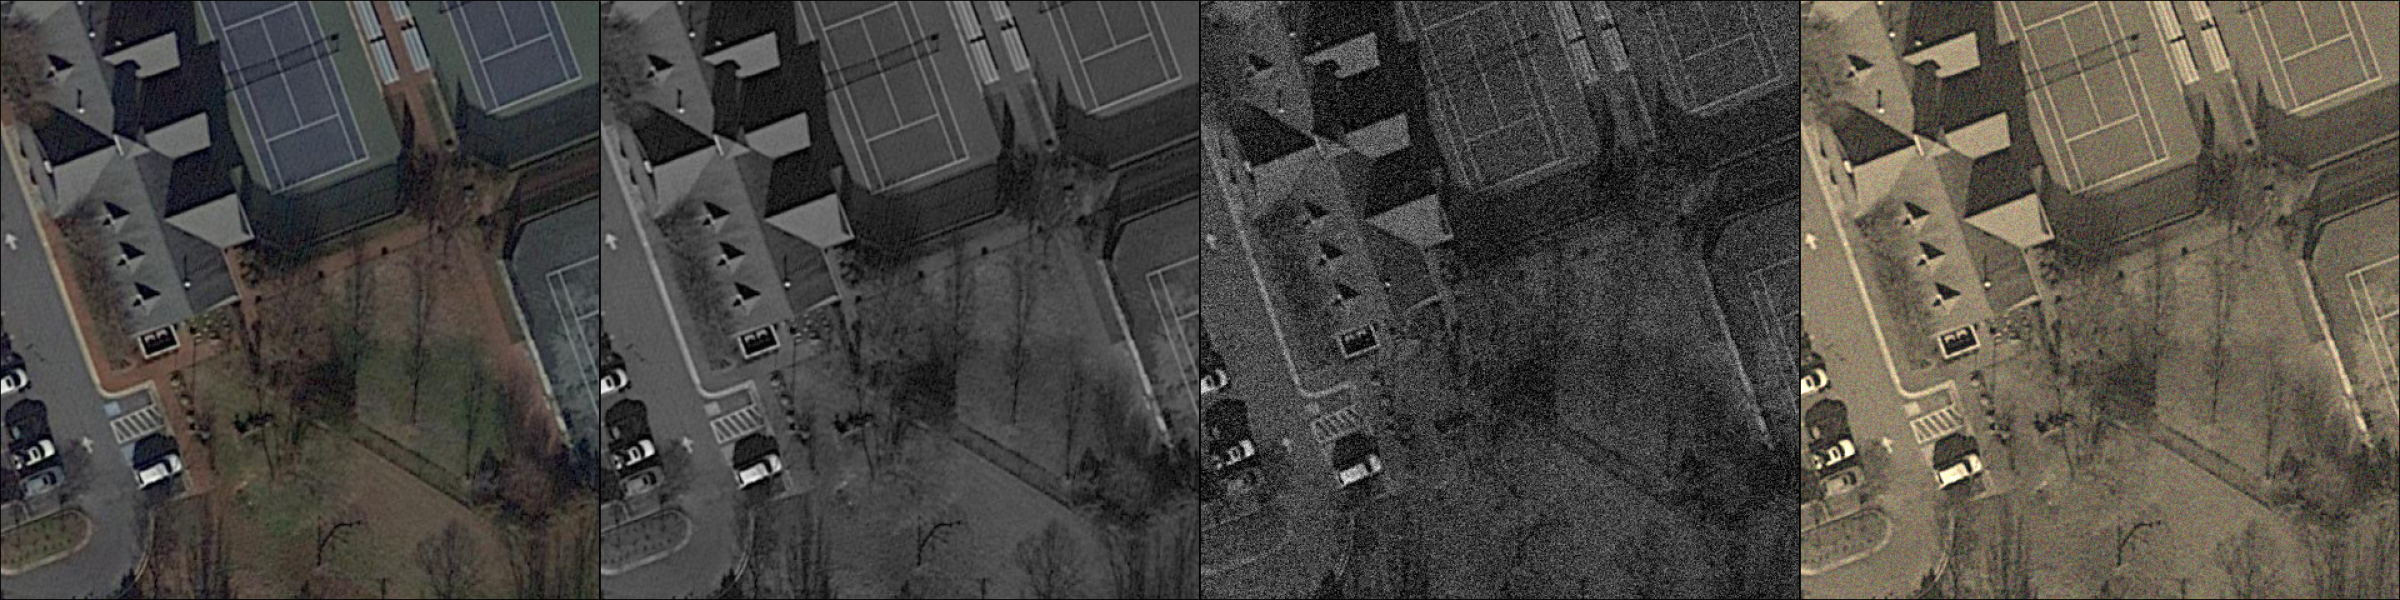
\includegraphics[width=0.9\textwidth]{Images/filters.png}
\caption{Comparison of original aerial image patch with three historic filter transformations: grayscale conversion, sepia toning, and Gaussian noise addition. These filters simulate common degradation patterns in historical aerial photography.}
\label{fig:historic_filters}
\end{figure}


% #############################################################################
\section{Final Dataset Statistics}

The completed Aerial-D dataset represents a comprehensive resource for aerial referring expression segmentation, containing over 1.5 million expressions across diverse object categories and linguistic patterns. As demonstrated in Figure \ref{fig:dataset_examples}, the final dataset showcases the broad range of instances, groups, and semantic categories enhanced through our multi-stage pipeline, with LLM-generated expressions providing rich visual details and contextual references that extend far beyond the original rule-based templates.

% Dataset examples figure
\begin{figure}[H]
\centering
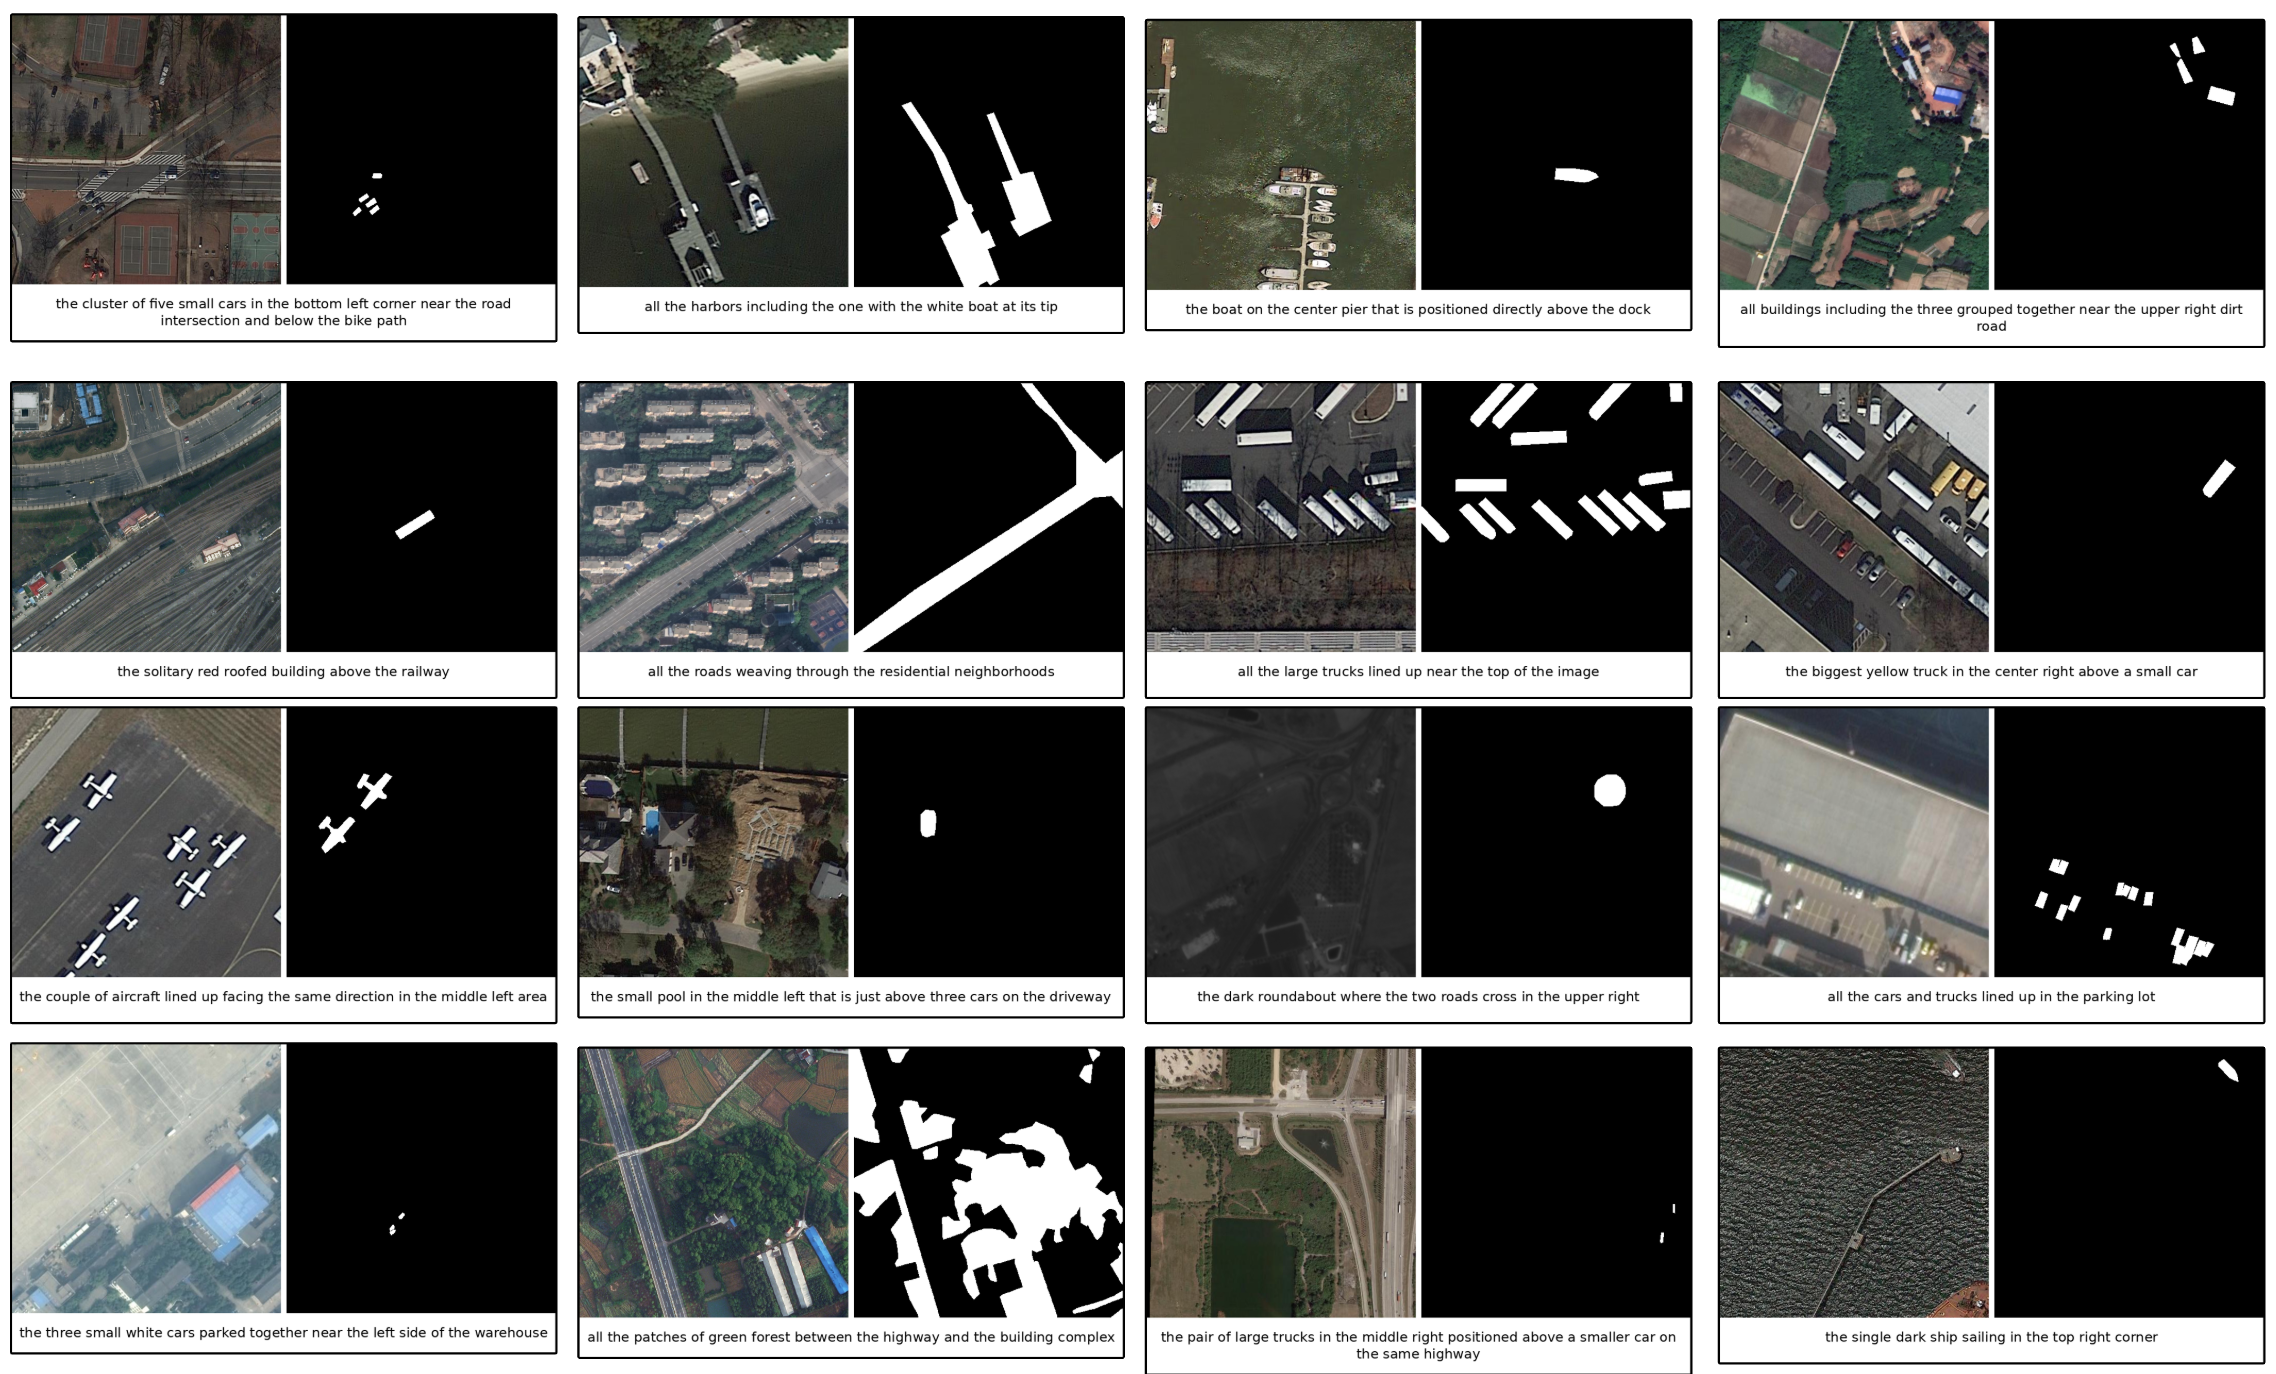
\includegraphics[width=\textwidth]{Images/dataset.png}
\caption{Representative examples from Aerial-D dataset showing diverse referring expressions with corresponding aerial images and ground truth masks.}
\label{fig:dataset_examples}
\end{figure}

Table \ref{tab:dataset_stats} presents the overall dataset composition, revealing 37,288 total patches containing 259,709 annotated samples with expressions. The dataset maintains a balanced distribution between individual objects (128,715 instances with 889,354 expressions) and groups (130,994 groups with 633,169 expressions), with an average of approximately 7 expressions per individual object and 5 expressions per group. The substantial scale demonstrates the comprehensive coverage achieved through our systematic generation pipeline.

% Dataset statistics table
\begin{table}[H]
\centering
\caption{Dataset Statistics Summary}
\label{tab:dataset_stats}
\begin{tabular}{@{}lrrr@{}}
\toprule
\textbf{Metric} & \textbf{Train} & \textbf{Val} & \textbf{Total} \\
\midrule
Total Patches & 27,480 & 9,808 & 37,288 \\
Individual Objects with Expressions & 94,179 & 34,536 & 128,715 \\
Individual Expressions & 646,686 & 242,668 & 889,354 \\
Groups with Expressions & 96,832 & 34,162 & 130,994 \\
Group Expressions & 471,108 & 162,061 & 633,169 \\
Total Samples & 191,011 & 68,698 & 259,709 \\
Avg. Expressions per Individual Object & 6.87 & 7.03 & 6.91 \\
Avg. Expressions per Group & 4.87 & 4.74 & 4.83 \\
\bottomrule
\end{tabular}
\end{table}

Category-specific statistics in Table \ref{tab:category_dist} illustrate the diversity across both iSAID and LoveDA source datasets, with small vehicles representing the most abundant category (41,353 individual instances) and specialized categories like helicopters and baseball diamonds providing targeted coverage for specific aerial object types. The distribution encompasses both discrete objects from iSAID and semantic land cover categories from LoveDA, ensuring comprehensive representation of aerial imagery content.

% Category distribution table
\begin{table}[H]
\centering
\caption{Object Category Distribution by Instance Type and Source Dataset}
\label{tab:category_dist}
\resizebox{\textwidth}{!}{%
\begin{tabular}{@{}lrrrrr@{}}
\toprule
\textbf{Category} & \textbf{Individual Instances} & \textbf{Groups} & \textbf{Instance Expressions} & \textbf{Group Expressions} & \textbf{Source Dataset} \\
\midrule
Small Vehicle & 41,353 & 53,682 & 262,831 & 282,848 & iSAID \\
Large Vehicle & 17,425 & 18,496 & 121,593 & 95,356 & iSAID \\
Ship & 11,461 & 10,402 & 79,251 & 49,272 & iSAID \\
Plane & 10,774 & 7,260 & 78,808 & 32,057 & iSAID \\
Harbor & 9,164 & 6,290 & 72,248 & 28,613 & iSAID \\
Tennis Court & 3,492 & 2,364 & 25,116 & 9,959 & iSAID \\
Bridge & 3,300 & 1,267 & 23,085 & 5,269 & iSAID \\
Swimming Pool & 3,147 & 1,999 & 23,355 & 10,011 & iSAID \\
Storage Tank & 2,985 & 3,451 & 19,537 & 16,071 & iSAID \\
Soccer Ball Field & 1,781 & 569 & 13,939 & 2,368 & iSAID \\
Ground Track Field & 1,368 & 208 & 9,111 & 868 & iSAID \\
Baseball Diamond & 1,049 & 381 & 7,965 & 1,576 & iSAID \\
Basketball Court & 959 & 636 & 7,339 & 2,757 & iSAID \\
Roundabout & 924 & 278 & 6,452 & 1,220 & iSAID \\
Helicopter & 354 & 266 & 2,636 & 1,144 & iSAID \\
Vehicle Pair & 0 & 7,597 & 0 & 30,388 & iSAID \\
Building & 10,341 & 3,012 & 66,038 & 12,048 & LoveDA \\
Water & 8,838 & 2,917 & 70,050 & 11,668 & LoveDA \\
Road & 0 & 3,018 & 0 & 12,072 & LoveDA \\
Forest & 0 & 2,850 & 0 & 11,400 & LoveDA \\
Agriculture & 0 & 2,342 & 0 & 9,368 & LoveDA \\
Barren & 0 & 1,709 & 0 & 6,836 & LoveDA \\
\bottomrule
\end{tabular}%
}
\end{table}

Table \ref{tab:expression_types} provides a detailed taxonomy of the 17 distinct expression templates used in rule-based generation, showing how combinations of category, position, extreme positioning, color, and relationship attributes create expressions ranging from simple category references to complex multi-attribute descriptions. The systematic enumeration demonstrates the comprehensive linguistic coverage achieved through combinatorial rule application.

% Expression taxonomy table with counts
\begin{table}[H]
\centering
\caption{Complete Taxonomy of Generated Expression Types}
\label{tab:expression_types}
\resizebox{\textwidth}{!}{%
\begin{tabular}{@{}cccccrl@{}}
\toprule
\textbf{Category} & \textbf{Position} & \textbf{Extreme} & \textbf{Color} & \textbf{Relationship} & \textbf{Total Count} & \textbf{Example} \\
\midrule
\multicolumn{7}{l}{\textbf{Individual Instance Expressions}} \\
\midrule
\checkmark & & & & & 5,157 & "the ship" \\
\checkmark & \checkmark & & & & 26,437 & "the ship in the bottom right" \\
\checkmark & \checkmark & & & \checkmark & 25,403 & "the ship in the bottom right that is to the left of a harbor" \\
\checkmark & & \checkmark & & & 22,930 & "the topmost ship" \\
\checkmark & \checkmark & \checkmark & & & 22,930 & "the topmost ship in the top left" \\
\checkmark & \checkmark & \checkmark & & \checkmark & 9,761 & "the topmost ship in the top left that is above a building" \\
\checkmark & & & \checkmark & & 19,172 & "the dark ship" \\
\checkmark & \checkmark & & \checkmark & & 58,252 & "the dark ship in the bottom right" \\
\checkmark & \checkmark & & \checkmark & \checkmark & 42,165 & "the dark ship in the bottom right that is to the left of a harbor" \\
\checkmark & & \checkmark & \checkmark & & 35,571 & "the dark topmost ship" \\
\checkmark & \checkmark & \checkmark & \checkmark & & 35,571 & "the dark topmost ship in the top left" \\
\checkmark & \checkmark & \checkmark & \checkmark & \checkmark & 15,242 & "the dark topmost ship in the top left that is above a building" \\
\midrule
\multicolumn{7}{l}{\textbf{Group Expressions}} \\
\midrule
\checkmark & \checkmark & & & & 40,281 & "the group of 3 ships in the center" \\
\checkmark & \checkmark & & & \checkmark & 86,307 & "the group of 3 ships in the center that is above a group of 2 buildings" \\
\checkmark & & & & & 61,015 & "all buildings in the image" \\
\bottomrule
\end{tabular}%
}
\end{table}

Finally, Table \ref{tab:llm_enhancement_stats} quantifies the impact of LLM enhancement, showing that the distillation pipeline successfully tripled the dataset size from the original 506,194 rule-based expressions to 1,522,523 total expressions. The LLM enhancement process contributed nearly equal numbers of language variations (496,895) and unique visual detail expressions (519,434), demonstrating the effectiveness of the two-pronged enhancement strategy in achieving both linguistic diversity and contextual richness.

% LLM enhancement stats table
\begin{table}[H]
\centering
\caption{LLM Enhancement Expression Distribution}
\label{tab:llm_enhancement_stats}
\begin{tabular}{@{}lrrr@{}}
\toprule
\textbf{Expression Source} & \textbf{Train} & \textbf{Val} & \textbf{Total} \\
\midrule
Rule-Based Expressions & 371,360 & 134,834 & 506,194 \\
LLM Enhanced (Language Variations) & 364,396 & 132,499 & 496,895 \\
LLM Unique (Visual Details) & 382,038 & 137,396 & 519,434 \\
\midrule
\textbf{Total Expressions} & \textbf{1,117,794} & \textbf{404,729} & \textbf{1,522,523} \\
\bottomrule
\end{tabular}
\end{table}

The construction of the Aerial-D dataset represents a significant advancement in aerial referring expression segmentation resources, providing comprehensive coverage of object categories, spatial relationships, and linguistic diversity. The resulting dataset serves as a foundation for training and evaluating sophisticated referring segmentation models that can understand complex natural language descriptions in aerial imagery contexts.
